\section{Workload Runtime and Placement (WRAP)}

\subsection{Overview}

WRAP concerns all aspects
of an \ngrm\ job, as it is allocated to and executed on compute resources
that are increasingly diverse, dynamic, distributed and large.
Stated very simply, the main problem domain of this thrust
area is $R \rightarrow J$: scheduling computing resources
with these properites ($R$) to a job ($J$) and providing services
to the job's processes for efficient execution. As we zoom in on
this high-level problem statement, however,
we find ourself facing a highly complex set of requirements
and use cases.

Untangling these complexities into solvable forms requires
rigorious conceptualization of our domain and
sound mechanisms that well embody the new concepts.
Given the magnitude of the problem domain, however, devising
solutions would need multiple iterations during
which we progressively tighten up the link between
the concepts and their mechanisms. New concepts that result from
the conceptualization efforts
should guide WRAP in proposing and developing
prototypes of certain mechanisms. Certain
mechanical reality learned from these mechanisms should then be
used to recalibrate their supporting concepts.
%Ultimately, how well our concepts address the overall 
%requirements and use cases and ease of mechanical realization 
%should determine the soundness of our solutions. 

As a first step towards this iterative process,
we propose a simple job model in the following that represents
our expanded notion of an job and its relations
to our generic compute resource model.
More specifically, our job model forms our basis to identify
resource management and runtime service primitives
from which to compose higher-level operations.
The primitives and high-level operations then
become our building blocks to relate a job
to its resources. We note that, however, our job model
assumes some properties on the generic
compute resource model at this point, as the resource management thrust is
currently conceiving the latter.
Finally, we will propose several WRAP mechanisms
and software architectures that can support the proposed job model.

\subsection{Hierarchical Job Model}

\begin{figure}
  \centering
    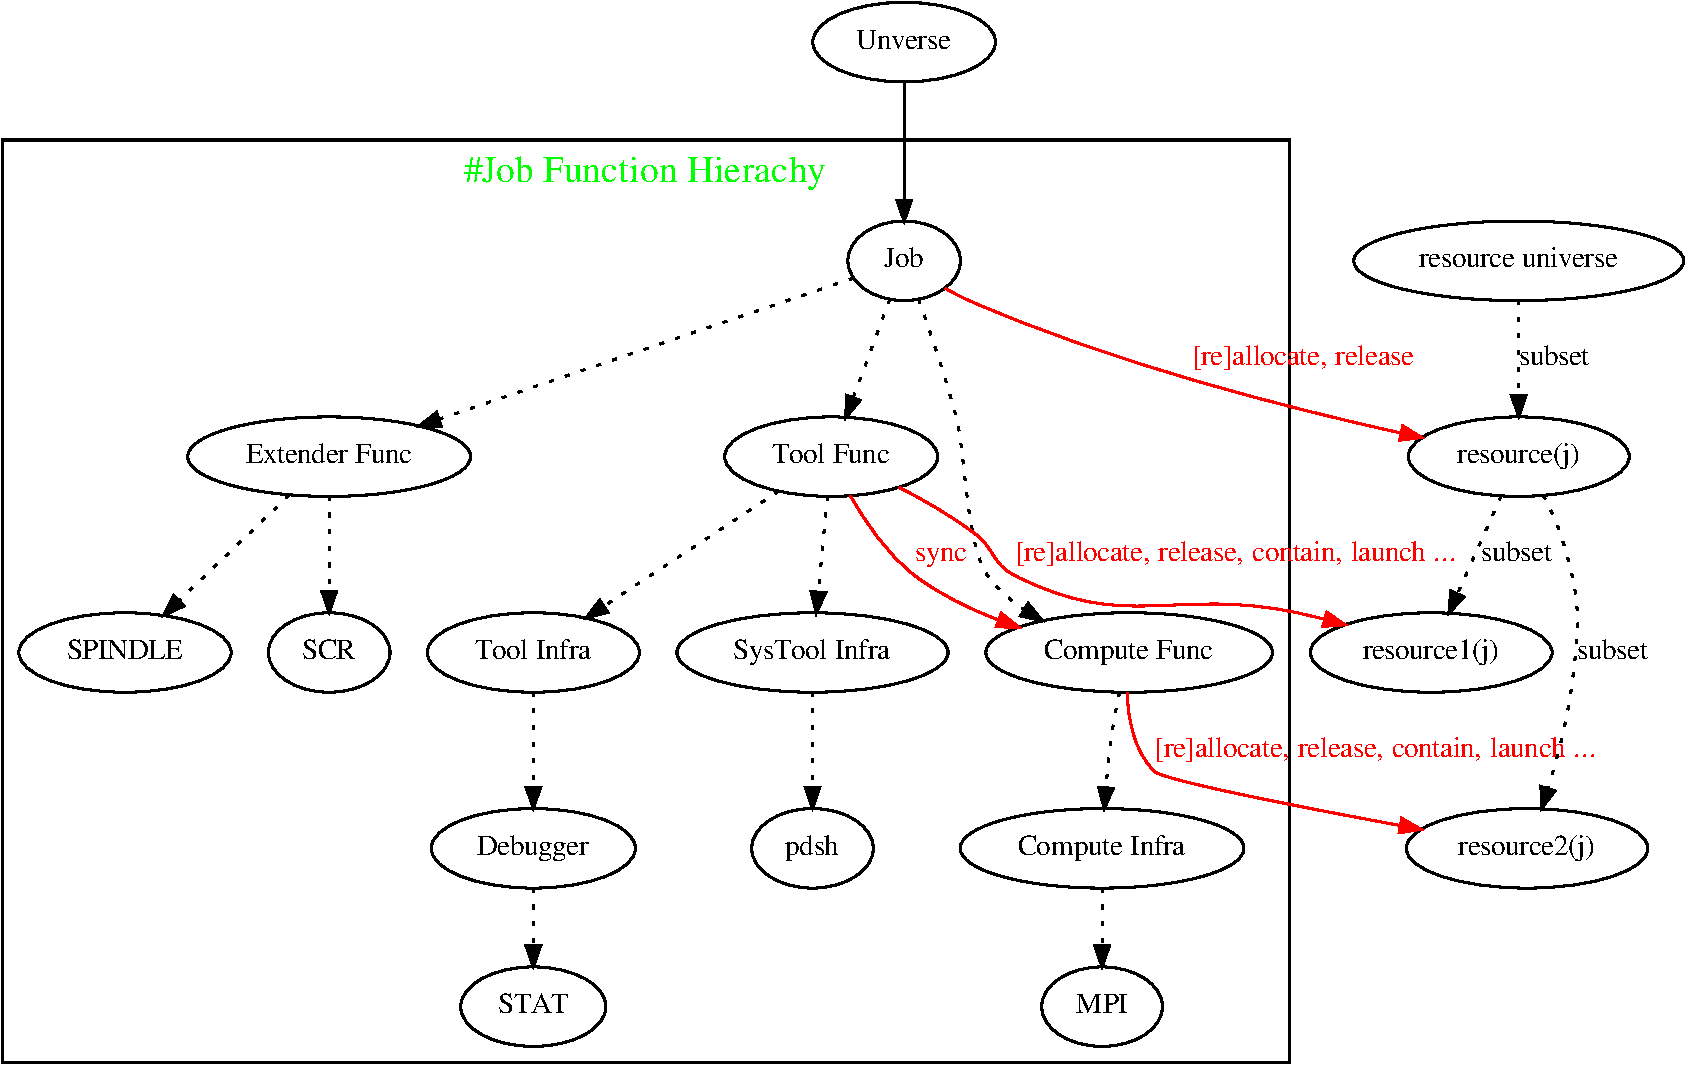
\includegraphics[width=5.0in]{wrap_graph}
  \caption{WRAP model on NGRM's $R \rightarrow $J problem}
  \label{fig:jobrm}
\end{figure}

Broadly speaking, today's resource management systems define a job as a set
of compute steps that are run on a fixed set of compute nodes with exclusive access for
a duration of time~\cite{Jette02slurm}.
This simple job model, however, is not flexible enough for our resource manager to
be able to express scheduling and runtime idioms required for the next generation computing systems.
Evidently, the job model already significantly limits
our resource manager's ability to address emerging
computing requirements and use cases.

Eliminating the limitations requires a more flexible notion that enables
our resource manager to organize and group the processes of a job
in accordance with their functions. For this purpose,
we introduce the notion of job functions. For example,
a job may need to create two disjoint sets of processes,
one for executing an MPI program and
the other for executing a parallel debugger program
that acts on the MPI program.
In this case, our system would want to group and manage the processes
that belong to each set separately. The notion of job functions
provide ways to organize those processes in two separate process management
domains. Simliarly, we may often need to organize
the set of processes within a same job function
into several smaller job functions. With the introduction of job functions,
a job becomes a set of job functions forming a hierarchy,
a hierarchical job model.

Using the new concept, our solution for the main
$R \rightarrow J$ problem can then be expressed as
providing effective services to schedule
a {\em job function hierarchy} to a resource allocation
that also forms a hierarchy as shown in
Figure~\ref{fig:jobrm}.
Our problem of $R \rightarrow J$ then becomes more than a traditional
resource allocation to a job. It is the problem associated with
resource distribution across the entire job function hierarchy.
Stated differently, the resource allocated to the root of the hierarchy
becomes the overall resource bound to the job functions at
the next level. This resource distribution relation is well defined
recursively for any job function at any position in the job hierarchy.

When we combine this hierarchical job model with our generic
compute resource model that can capture a wide range
of compute resources from fixed resources such as compute nodes
and software licenses, to consumable resources like power,
we realize that we can express a vastly rich set
of scheduling and runtime idioms.
The following builds basic definitions and formalisms
to reason about our hierarchical job model with some mathematical rigor.
They are our tool to compose more complex concepts
and to test the concepts on the requirements and use cases
of the next generation resource management.

\begin{table}
\centering
\begin{tabular}{|l|l|}
\hline
Term & Description \\
\hline
$u$ & universe  \\
$r_u$ & a set of resources allocated to $u$ \\
$j$ & a job or job function in a specific job hierarchy \\
$parent(j)$ & $j$'s parent in its job hierarchy ($parent(root)$ = $u$) \\
$c_j$ & resource criteria for $j$ \\
$d_j$ & some data to record by $j$ \\
$r_j$ & a set of compute resources allocated to $j$ where $r_j \subseteq r_{parent(j)}$ \\
$cnew_j$ & criteria for additional resources for $j$ \\
$rnew_j$ & a set of additional resources where $rnew_j \not\subseteq r_j$ and $rnew_j \subseteq r_{parent(j)}$ \\
$e_x$ & a runtime environment where $e_x \in E = \{e0, e1, ..., e_{m-1}\}$ \\
\hline
\end{tabular}
\caption{Basic definitions for our job model}
\label{tab:def}
\end{table}

\subsubsection{WRAP Service Primitives}
\label{sect:prim}

Table~\ref{tab:def} describes the basic elements of our job model, representing
the nodes in Figure~\ref{fig:jobrm}. For example, $j$ represents any node
in the job hierarchy graph and similarly $r$ represents any node in the resource hierarchy graph.
Using those as the foundational concepts, we propose
the following WRAP service primitives as the conceptual means
needed for $r_j \rightarrow j$:

\begin{itemize}

\item{$alloc(j, c_j)$: allocates $r_j$ to $j$ from $r_{parent(j)}$ according to $c_j$.}

\item{$realloc(j, cnew_j)$: allocates $rnew_j$ from $r_{parent(j)}$ according to $cnew_j$ and updates $r_j$ such that $r_j = r_j \cup rnew_j$.}

\item{$release(j, subset(r_j))$: releases a subset of $r_j$ to $r_{parent(j)}$ and updates $r_j$ such that $r_j = r_j - subset(r_j)$.}

\item{$contain(j, e_x)$: contains $j$ in $e_x$.}

\item{$launch(j)$: spawns, maps and binds processes of $j$ on $r_j$ according to $c_j$. If this is an incremental launch, this spawns and binds only additional processes.}

\item{$destroy(j)$: kill processes of $j$ running on $r_j$. If this is a partial destory, this kills only a subset of processes.}

\item{$bootstrap(j)$: bootstraps processes of $j$ across $r_j$ including dissemination of connection information. If this is a partial bootstrap--e.g., additional processes have been spawned or some processes have been killed, it only adjusts $j$ for the change}

\item{$split(j, marker)$: creates a new job function that includes all of the calling processes of $j$ with the same marker.}

\item{$record(j, d_j)$: records $j$'s attributes such as its $c_j$, fingerprint for $e_x$, and arbitrary information ($d_j$).}

\item{$query(j)$: queries about $j$.}

\item{$sync(j_k, j_l)$: putting a job function $j_k$ into a known state and providing another job function $j_l$ with $j_k$'s identify info.}

\end{itemize}

\subsubsection{Higher Level Operations}
\label{sect:hiop}
We now build some of common high-level services
by composing service primitives in Section~\ref{sect:prim}.

\begin{itemize}

\item{$init(j, c_j)$ = $<alloc(j, c_j), launch(j), bootstrap(j)>$}

\item{$cont\_init(j, c_j, e_x)$ = $< alloc(j, c_j), contain(j, e_x), launch(j), bootstrap(j) >$}

\item{$grow(j, cnew_j)$ = $<realloc(j, cnew_j), [launch(j), bootstrap(j)]>$,  where $launch$ and $bootstrap$ are only needed when $grow$ needs to launch additional processes. For instance, if $cnew_j$ is a power bound increase request, these operations are unnecessary.}

\item{$shrink(j,subset(r_j)$ = $<release(j, subset(r_j)), [destroy(j), bootstrap(j)]>$, where $destroy$ and $bootstrap$ are only needed when $shrink$ needs to kill some processes of $j$.}

\item{$monitor(j, j_{mon}, c_j)$ = $<init(j, c_j), init(j_{mon}, c_j), sync(j, j_{mon})>$, where the first $init$ should be passed a special flag to cooperate with the subsequent $sync$ operation.}

\item{$log(j, j_{logger}, c_j)$ = $<init(j, c_j), init(j_{logger}, c_j), sync(j, j_{logger})>$, where the first $init$ should be passed a special flag to cooperate with the subsequent $sync$.}

\end{itemize}

\subsection{Composed Use Cases}
We now show the expressibility of the service primitives and
high-level operations by mapping them to some of the
use cases of the next generation resource management.

\begin{itemize}

\item{UC1: Use NGRM recursive execution to manage dedicated application test time.

$<alloc(j, c_j), alloc(j_{t0}, c_{j_{t0}}), alloc(j_{t1}, c_{j_{t1}}), ...>$, where each $r_{j_i}$ represents distinct set of resources in $r_{j}$ and each $j_{ti}$ can further run a specific test under a different environment using services like $cont\_init$.}

\item{UC3-UC5: Power utilization as a resource etc.

We must combine our job model to the generic resource model to express these use cases.}

\item{UC6: Live user feedback for job progress.

$monitor(j, j_{progress\_monitor})$.}

\item{UC7: Allow users to inject application specific data into data stream for jobs.

$<initialize(j, c_j), record(j, d_j)>$.}

\item{UC8: dsh|dshbak.

I.e., $<init(j, c_j), init(j_{dsh}, c_j)>$}.

\item{UC9: User control over system software levels.

I.e., $<cont\_init(j, c_j, e_{prev.lvl}), record(j, d_j)>$.}

\item{UC10: Testing system software releases.

I.e., $<cont\_init(j, c_j,e_{toss.v}), record(j, d_j)>$.}

\item{UC11: Integrated tool support.

I.e., $<init(j, c_j), init(j_{STAT}, c_j), sync(j, j_{STAT})>$.}

\item{UC12: Allocate spare resources from a common pool.

I.e., $<init(j, c_j), grow(j_{scr}, cnew_j), sync(j, j_{scr})>$.}

\item{UC12.1: Allocate additional power for some critial code region.

I.e., $<init(j, c_j), grow(j, cnew_j), shrink(j)>$.}

\item{UC13: Checkpoint/restart,

I.e., $<init(j, c_j), init(j_{scr}, c_j), sync(j, j_{scr})>$.}

\item{UC14: Ephemeral file system instances.

We must combine our job model to the generic resource model to express these use cases.}

\item{UC15: Integrated I/O forwarding support.

$<alloc(j, c_j), init(j_{mpi}, c_{j_{mpi}}), init(j_{iof}, c_{iof}), sync(j_{mpi}, j_{iof})>$.}

\item{UC16: Hadoop framework.

$<init(j_{hadoop}, c_{j_{hadoop}})>$.}

\item{UC17: User database instances.

I.e., $<init(j_{mysql}, c_{j_{mysql}}), init(j_{atool}, c_{j_{atool}}), sync(j_{mysql}, c_{j_{atool}})>$.}

\item{UC20: Provide "pre-job" resource information.

$<alloc(j, c_j), query(j), init(j_{mpi}, c_{j_{mpi}})>$.}

\item{UC19: Record HW configuration.

$<init(j, c_j), record(j, d_j)>$.}

\item{UC21: Virtual private networks for jobs.

$<cont\_init(j, c_j, e_{vpn})>$.}

\end{itemize}

\subsubsection{Advanced Power-Aware scheduling Support}
Our hierarchical job model allows varying grain of control for both the size of
a job function (in terms of its process count) and resource distribution
across the job functions.
That has many interesting properties. For example, an MPI
job function can further break itself down into smaller job functions
representing groups of MPI processes or even smallest functions:
individual MPI processes as job functions.
As smaller functions allocate, grow or shrink within the resource
bound allocated to their parent MPI job function, consumable resources
like power can be unevenly or evenly distributed across
those smaller functions.
This concept can well support LLNL's power-aware scheduling research.

\subsection{WRAP Software Architecture and Mechanisms}
\label{sect:arch}
\begin{figure}
  \centering
    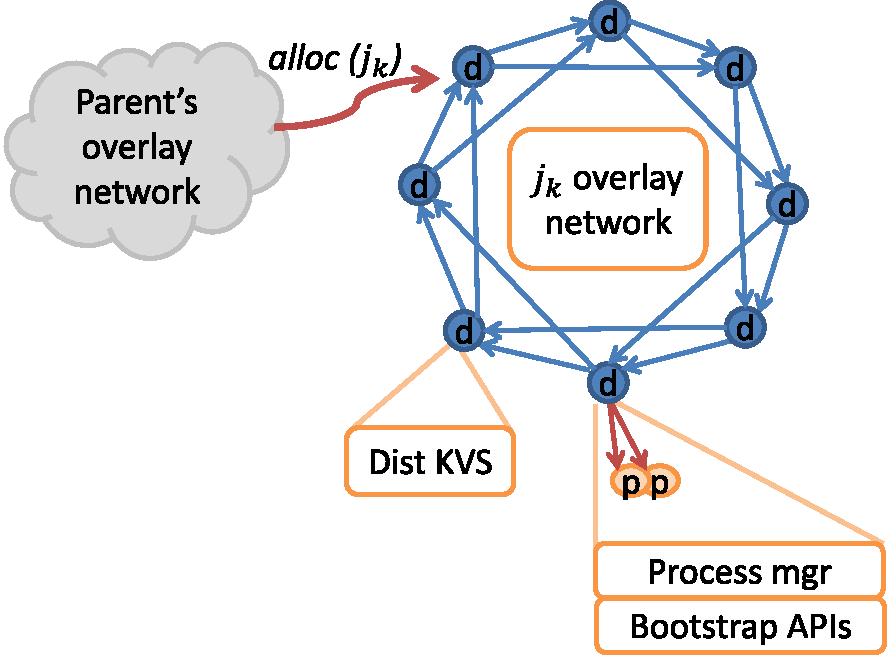
\includegraphics[width=3.0in]{WRAP_Base}
  \caption{Base WRAP architecture for $alloc(j_k, c_{j_k})$}
  \label{fig:base}
\end{figure}
In this section, we propose our WRAP software architecture and mechanisms
that can support scheduling generic compute resources to our hierarchical job
model. We will first describe the base architecture designed to support
compute nodes as the resource type. Next, we will extend that architecture
to embody more advanced concepts such as synchronizing job functions,
growing compute nodes allocated to an existing job function and further
handling other types of resources such as power.

\subsubsection{Base WRAP Architecture to Schedule a Single Job Function}
Figure~\ref{fig:base} shows our base software architecture
that can provide a single job function ($j_k$) with service primitives:
$alloc()$,
$launch()$,
$bootstrap()$,
$contain()$,
$record()$, and
$query()$.
It assumes that the overlay network of $parent(j_k)$
already exists and that it can instantiate a highly scalable,
resource-efficient overlay network for $j_k$ upon
granting the $alloc(j_k)$ request. In fact, our architeture
requires that any overlay network instance recursively
supports communications of a child job function either
through an explicit instantiation of a separate overlay network
or through the existing overlay network. The latter model,
however, requires to support a growth and/or reconfiguration
of the existing network to be flexible.
WRAP then uses the overlay network of $j_k$ as well as
a key-value store to serve process management scalably
to $j_k$'s processes.
The following explains key process management services
and distributed key-value store mechanisms in detail.

\paragraph{Process Management (ProcMan) Services}
\label{sect:procman}

\begin{itemize}
\item{{\bf Bulk Process Creation and Stop}: The head daemon of the overlay network
receives a process creation request
through $launch(j_k, c_{j_k})$ and propagates that command to the rest of the daemons
in $O(log(N))$. Upon receiving the request, each daemon forks and execs
local processes. If the request contains an optional {\tt sync\_assist} flag, the daemons
stop the processes immediately after the creation to support a subsequent $sync()$ issued
by another job function. In either case, the daemons store
information on the created target processes such as their process id, executable path
and hostname, into a distributed key-value store that will be explained later.}

\item{{\bf Scalable Propagation of Environments}: The head daemon receives the environment
variables list and propagates that to the rest of the deamons
in $O(log(N))$. The daemons then concatenate this master environment variables
list to their local environment variables and export them to their
processes. If the head daemon receives an optional $contain$ request, that
request is also being propagated. The specified containing-environment is used to contain
the target processes.}

\item{{\bf Process Mapping and Binding}: The daemons provide the newly created processes
with topology information to support their mapping and binding to the underlying 
resources. The daemons retrieve the topology information from the key-value store.}

\item{{\bf Scalable {\tt stderr/stdout} Handling}: The daemons receive
{\tt stderr} and {\tt stdout}
from their processes and scalably push and merge them through a tree in the overlay
network towards the head daemon. Output aggregation techniques
will include ways to reduce the output progressively at every merge step
in the tree either by applying a readily available
reduction filter or a user-provided one.}

\item{{\bf Scalable signal/{\tt stdin} Forwarding}: The head daemon receives a UNIX signal
or an input through {\tt stdin} and scalably propagates it to a specified set of daemons
through a tree in the overlay network in $O(log(N))$. Upon receiving the signal or {\tt stdin},
each daemon routes it to their corresponding processes.}

\item{{\bf Scalable Process Termination Detection and Analysis}: When one or more processes
in the job function are normally or abnormally terminated, their home daemons detect the event and notify
the head daemon through a tree in the overlay network. A time-out filter can be used at every step of
the tree network to merge the return codes and, if abnormal, the stack traces of 
the terminated processes. Upon receiving the aggregated
event, the head daemon will clean up the entire job function and also present
to the users concise information about the termination.}

\end{itemize}

\paragraph{Distributed Key-Value Store (DKVS) for Scalable Global Information Sharing}
\label{sect:dkvs}

DKVS provides a scalable mechanism by which the processes of $j_k$ can
share arbitrary information in a key-value pair among them.
Conceptually, DKVS represents a global key-value tuple space
and any process of $j_k$ can store its data by associating them
with a unique key. To be memory-efficient,
however, DKVS must store the data in a distributed
manner. Thus, the overlay network of $j_k$ is capable of hashing the key
to route its tuple to the home key-value store location. Global synchonization
mechanisms such as collective fense will be provided to force
memory consistency of DKVS across all processes.

Because our overlay network will have built-in routing
schemes, the actual database we will use can be simple.
Thus, we will first consider a readily available, simple
database such as {\tt Redis} with no internal distribution support.
Depending on our overlay network topology,
KVS can be fully distributed across all of the overlay network daemons.
An example topology is a forest
with $log(N)$ connections wherein any daemon can be
the root of a binomial tree.

Our DKVS will support a hierarchical tuple space for better
data encapsulation per job function, leading to a higher level of security and protection.
More specifically, when a job function is
allocated, a new name scope for that job function will be
created and information on the resource allocated
to that job function will be stored as part of the default $record$ service: e.g.,
$j_k$::resource $\rightarrow$ $<$ core\_count(1024), power\_bound(100kw), ... $>$.
This information is accessible by $j_k$ as well as
its immediate child job function $j_{k+1}$.
Similarly, when a daemon creates an MPI rank process, it will add the
personality of that process under this job function name scope
such as $j_k$::rank(128) $\rightarrow$ $<$ host IP, pid, executable path, ... $>$.
Finally, DKVS will allow any process of the job function to store arbitrary data
as part of $record(j_k, d_{j_k})$. All information stored
as part of $record$ will be pushed to $parent(j_k)$ when $j_k$
is destroyed. Thus, the information will ultimately find its place
in a persistent resource manager database. In addition,
DKVS will further support $query$, providing the calling process
with underlying resource allocation infomation.

\paragraph{Unified Mechanism to Support Various Distributed Software Bootstrap Interfaces}
\label{sect:bootstrap}

DKVS will be designed to support a wide range of bootstrap interfaces
for distributed software including PMI 1 and 2~\cite{PMI2}, PMGR Collective and COBO,
LaunchMON~\cite{launchmon} and LIBI~\cite{libi}. With support for these interfaces
WRAP will be able to bootstrap a wide range of job functions including a myriad of
MPI implementations, tools communication infrastructure such as MRNet
and also end-user tools such as STAT, TotalView and OpenSpeedShop.
Specifically, the PMI layers will be a very thin layer on top
of our DKVS implementation. We will support PMGR Collective,
COBO, LaunchMON, and LIBI such that each created process opens
up an ephemeral TCP port and store it as $j_k$::rank(128) $\rightarrow$ $<$ host IP, port $>$.
Then, each process in the binomial tree in these bootstrappers
will simply find the connection information of its parent as well as
its children using their ranks as the keys.

\subsubsection{Architectural Support for Job Function Synchronizations}
\label{sect:sync}
Our hierarchical job model has an ability to relate a job function
to another through $sync$.
For example, a tool may need to be co-located with an MPI job
and attached to its processes.
Thus, we must extend our base architecture to support that concept.
\begin{figure}
  \centering
    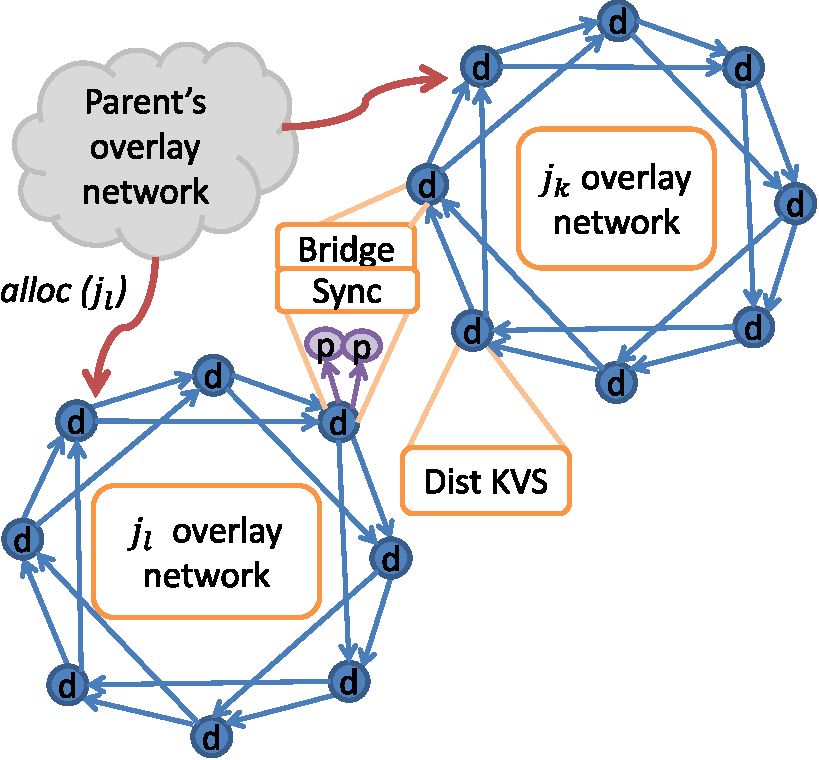
\includegraphics[width=3.0in]{WRAP_newJobFunction}
  \caption{WRAP architecture support for ${sync(j_k, j_l)}$}
  \label{syncext}
\end{figure}
As shown in Figure~\ref{syncext}, when $alloc(j_l)$
is granted for an additional new job function $j_l$,
the parent overlay network instantiates
another overlay nework for $j_l$ and helps manage
the processes of $j_l$ in the same manner as the base case.
To support ${sync(j_k, j_l)}$,
however, a connection needs to be made beween $j_l$'s
overlay and $j_k$'s overlay network.
For this purpose, we introduce the concept
of bridge. The bridge allows processes
of $j_l$ to be able to access DKVS of $j_k$, which includes
the mapping of the global MPI rank of a process of $j_k$
to its host name, pid, executable path~\cite{MPIRInterface},
information necessary for $j_l$ to locate all of $j_k$'s processes.
Alternatively, if the existing overlay network of $j_k$ is
capable of allocating and managing a new sibling job function
within itself, the need for a connection between two overlay
network and DKVS is eliminated.

\subsubsection{Architectural Support for Reallocation of Compute Nodes}
Our hierachical job model includes an ability to grow a job function $j_k$
by reallocating a new set of resources from the resources allocated
to $parent(j_k)$ and launching and bootstraping additional processes
across them.
Figure~\ref{fig:ext2} shows architectural support for that
job model.
\begin{figure}
  \centering
    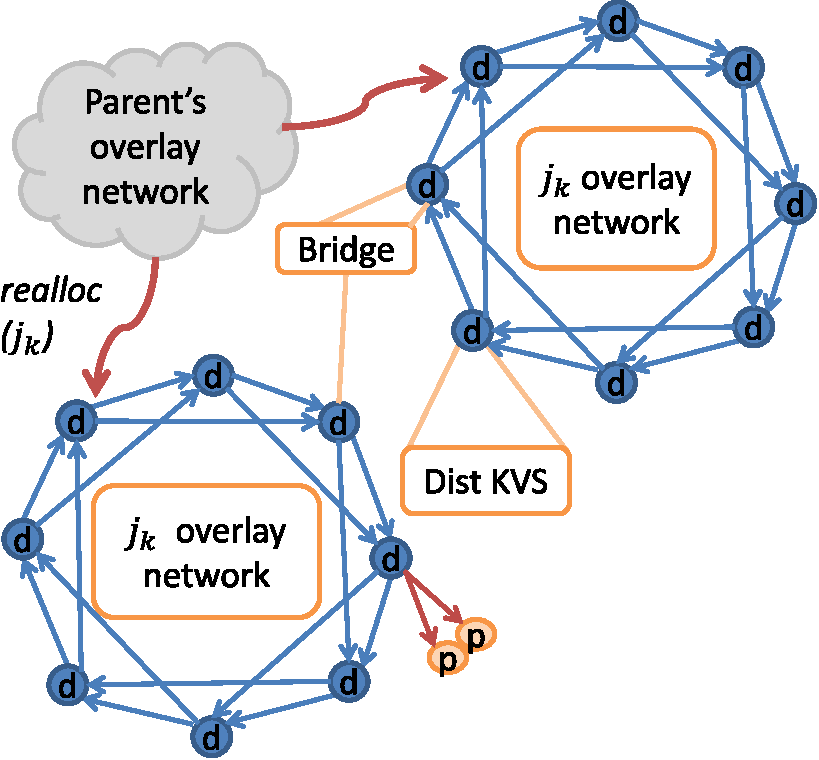
\includegraphics[width=3.0in]{WRAP_grow}
  \caption{WRAP architecture support for ${grow(j, cnew_j)}$}
  \label{fig:ext2}
\end{figure}
The scheme is essentially the same as that of $sync$.
Upon granting a reallocation of $rnew_j$,
$parent(j_k)$'s overlay network instantiates an overlay network
across $rnew_j$ and connects it to the existing overlay network
of $j_k$. The bridge support is again central for the connection.
Additional processes launched through the new network will
be able to access the DKVS associated with the existing $j_k$
name scope. Conversely, DKVS associated with these additional
processes will be made available to the existing $j_k$.
Alternatively, if the existing overlay network of $j_k$ is
capable of allocating and managing these additional processes
within itself, the need for a connection between two overlay
network and DKVS is eliminated. However, the existing overlay network
of $j_k$ is required to be capable of growing and
reconfiguring itself to cover the additional compute nodes.

\subsubsection{Architectural Support for Power as a Resource Type}
As $j$ will get the power bound allocated as a resource type,
a power control mechanism like RAPL~\cite{RountreeRAPL} can be used
to set the power bound of the allocated compute nodes.
The basic scheme computes the per-node power-bound average
and sets that averaged bound on each compute node.
For more advanced power-aware scheduling, groups of processes will
be assigned to new "power-domain" job functions using $split()$.
The new power-domain job functions will use $grow()$ and $shrink()$
operations described in Section~\ref{sect:hiop}
on the power bound as the resource type.
Although the distribution of power bound across compute
nodes will vary, our scheme will guarantee the aggregate power use
across all of these "power-domain" job functions bounded to the overall power bound
allocated to their parent.
These new job functions will create new name scopes
in the DKVS under their parent name scope:
e.g., $j_k$::$j_{k+1}$::resource $\rightarrow$ $<$ size(128), power\_bound(12.5kW) $>$.

\subsection{Component-Wise Work Breakdown}
In this section, we summarize the requirements and work items for
the major components of the proposed system.

\subsubsection{Overlay Network and Infrastructure Requirements}
The heart of WRAP lies in scalable and flexible overlay network support.
The overlay network's attributes that WRAP requires include:

\begin{itemize}

\item{an ability to support our elasticity model
efficiently and scalably through expanding and shrinking
compute nodes and job function processes launched on them;}

\item{an ability for an arbitrary head daemon to broadcast
or multicast data to a set of other daemons through a binomial
or binary tree with $O(log(number\_of\_daemons))$;}

\item{an ability for an arbitrary head daemon to aggregate data
sent from a set of other daemons through the binomial
or binary tree with $O(log(number\_of\_daemons))$;}

\item{an ability to allow both preset and custom-made reduction
opertators to reduce the aggregated data along the tree;}

\item{an ability to control data aggregation and reduction synchronously
with a mechanism to set an arbitrary time-out threshold: zero time-out means pass-through;
infinity time-out means global synchronization; and
in-between means partial synchronization with varying degrees;}

\item{an ability to route a key-value pair efficiently and
scalably by automatically hashing its key to find its home DKVS server
in support of get/put and global memory synchronization operations.}

\end{itemize}

\subsubsection{Process management}
To support scalable process management service described in Section~\ref{sect:procman},
the following components need to be investigated, designed and implemented:
\begin{itemize}
\item{an extensible communication protocol that allows
our process manager to conduct command and control
for all of its services;}
\item{a common data aggregation and reduction framework, techniques and API;}
\item{process management service components that
make use of the communication protocol and aggregation and reduction framework/API
and expose the services through high-level APIs;}
\item{executable commands such as a job function launcher that combines the
service components to implement certain types of process management
services for users;}
\item{topology-awared process binding and mapping components as well as
communication mapping APIs that client software can use for efficient
mappings between its communication patterns and the topology.}
\end{itemize}

\subsubsection{DKVS}
DKVS requires the following components:
\begin{itemize}
\item{name scoping specification and API;}
\item{direct get/put methods on a readily-available key-value server;}
\item{remote get/put methods on distributed key-value servers by
integrating servers to the communication infrastructure;}
\item{synchronization mechanisms and APIs that guarantee memory consistency
acorss the distributed servers.}
\end{itemize}

\subsubsection{Bootstrap Interfaces}
The following components should be implemented and demonstrated
using DKVS support:
\begin{itemize}
\item{PMI2 and port a version of MPICH as a reference implementation;}
\item{PMGR Collective and/or COBO and port a version of MVAPICH as a reference implementation;}
\item{LIBI and port a version of LIBI-enabled MRNet as a reference implementation.}
\end{itemize}

\subsubsection{Job Function Synchronization}
\begin{itemize}
\item{{\tt MPIR\_proctable} gatherer that gathers {\tt MPIR\_proctable} spread throughout the
DKVS into a centeral location including the address space of the job function launcher;}
\item{MPIR debug interface~\cite{MPIRInterface} that makes use of DKVS and process
management services to support parallel debuggers;}
\item{co-locator that co-locates an additional job function's processes with
the target processes;}
\item{LaunchMON Back-end API that makes use of DKVS to allow another job function processes
to discover the locations of target processes scalably.}
\end{itemize}

\subsubsection{Power Bound and Scheduling}
\begin{itemize}
\item{{\em split()} that allows an MPI job function to create smaller job functions, each with independent power bound control;}
\item{Dynamic power bound controller that manages expanding and shrinking of power bounds across these job functions.}
\end{itemize}

\subsection{Phase-Based Work Breakdown}
To bring up the proposed WRAP system progressively and expediently, we use a phased approach.
WRAP requires four phases: the outcome of earlier phases becomes the fundamental 
building blocks for the later phases.

\subsubsection{Phase 1: Basic Building Blocks (BBB) design}

\begin{table}
\centering
\begin{tabular}{|l|l|l|l|}
\hline
Work Item & Description & Dependency & Deliverable \\
\hline
\multirow{2}{*}{Protocol design} & design/prototype procMan & \multirow{2}{*}{comm. co-design} & \multirow{2}{*}{paper and review} \\
& command/control comm. protocol & & \\ \hline
\multirow{2}{*}{Aggregation/reduction design} & design/prototype aggregation &  \multirow{2}{*}{comm. co-design} & \multirow{2}{*}{paper and review} \\
& reduction framework and APIs & & \\ \hline
\multirow{2}{*}{DKVS name scoping design} & design/prototype name scoping & \multirow{2}{*}{comm. co-design} & \multirow{2}{*}{paper and review} \\
& specification and APIs & & \\ \hline
\multirow{3}{*}{Key-value store investigation}& evaluate key-value store servers & \multirow{3}{*}{none} & \multirow{3}{*}{finding summary} \\
& via direct put/get methods using & & \\
& bootstrap and MPIR emulation& & \\ \hline
\multirow{2}{*}{Power controller investigation} & investigate Intel RAPL &  \multirow{2}{*}{RM design} & \multirow{2}{*}{paper and review} \\
& and ways to control power bound & & \\ \hline
\end{tabular}
\caption{Phase 1 BBB design milestones and deliverables}
\label{tab:phase1}
\end{table}

During this phase, we will design and prototype the basic building blocks required
by WRAP. This layer represents the lowest building blocks for the WRAP thrust and has fundamental
dependecies on the overlay network infrastructure design as shown in Table~\ref{tab:phase1}.
Thus, they must be co-designed.

\subsubsection{Phase 2: Service Building Blocks (SBB) design and BBB implementation}
\begin{table}
\centering
\begin{tabular}{|l|l|l|l|}
\hline
Work Item & Description & Dependency & Deliverable \\
\hline
\multirow{2}{*}{ProcMan design} & design/prototype process manager & \multirow{2}{*}{comm. infra} & \multirow{2}{*}{paper and review} \\
& package and APIs & & \\ \hline
\multirow{2}{*}{Topo-aware binding design} & design/prototype topo-aware binding & \multirow{2}{*}{RM design} & \multirow{2}{*}{paper and review} \\
& and mapping mechanisms and APIs & & \\ \hline
\multirow{3}{*}{Remote DKVS} & investigate DKVS via & \multirow{3}{*}{comm. infra} & \multirow{3}{*}{finding summary} \\
& remote put/get/sync using bootstrap & & \\
& and MPIR emulation & & \\ \hline
\multirow{5}{*}{BBB Implementation} & implement ProcMan comm. protocol & \multirow{5}{*}{BBB proto} & \multirow{5}{*}{software drop} \\
& aggregation/reduction framework and API & & \\
& DKVS name scoping API & & \\
& direct key-value store & & \\
& power controller & & \\ \hline
\end{tabular}
\caption{Phase 2 SBB design milestones and deliverables}
\label{tab:phase2}
\end{table}

During this phase, we will use the design and prototypes of basic building blocks
to design and prototype higher-level service layer called service building blocks (SBB)
packages. In addition, that effort will further validate the BBB design and prototypes
and hence we will lock in the BBB design and produce production-quality BBB implementations
during this phase.
As shown in Table~\ref{tab:phase2}, this phase is designed to provide core WRAP functionality
engine except for the actual user interfaces to expose.

\subsubsection{Phase 3: User Service Interfaces (USI) design and SBB implementation}
\begin{table}
\centering
\begin{tabular}{|l|l|l|l|}
\hline
Work Item & Description & Dependency & Deliverable \\
\hline
\multirow{2}{*}{Job function utility design} & design/prototype job function utilities such & \multirow{2}{*}{SBB proto} & \multirow{2}{*}{paper and review} \\
& as job function launcher & & \\ \hline
\multirow{2}{*}{Job function sync design} & design/prototype job function & \multirow{2}{*}{SBB proto} & \multirow{2}{*}{paper and review} \\
& synchronizers & & \\ \hline
\multirow{2}{*}{PMI2, PMGR, LIBI design} & design/prototype boostrapers: & \multirow{2}{*}{SBB proto} & \multirow{2}{*}{finding summary} \\
& PMI2, PMGR/COBO and LIBI & & \\ \hline
\multirow{3}{*}{SBB implementation} & implement ProcMan package & \multirow{3}{*}{SBB proto} & \multirow{3}{*}{software drop} \\
& Topology-aware binding & & \\
& Remote DKVS & & \\ \hline
\end{tabular}
\caption{Phase 3 USI design milestones and deliverables}
\label{tab:phase3}
\end{table}

During this phase, we will use the design and prototype of service building blocks
to design and prototype the user-visible service layer called user service interfaces (USI).
In addition, once SBB prototypes are demonstrated that they are well-suited for the designed USI,
we will lock in the SBB design and produce production-quality SBB implementations.
As shown in Table~\ref{tab:phase3},
this phase will lay out the design of WRAP's external interfaces.

\subsubsection{Phase 4: USI implementation}
\begin{table}
\centering
\begin{tabular}{|l|l|l|l|}
\hline
Work Item & Description & Dependency & Deliverable \\
\hline
\multirow{2}{*}{Job function utility implementation} & implement job function& \multirow{2}{*}{NGRM framework} & \multirow{2}{*}{software drop} \\
& utilities such as launcher & & \\ \hline
\multirow{2}{*}{Job function sync implementation} & implement job function& \multirow{2}{*}{NGRM framework} & \multirow{2}{*}{software drop} \\
& job function synchronization & & \\ \hline
\multirow{2}{*}{PMI2, PMGR, LIBI design} & implement & \multirow{2}{*}{NGRM framework} & \multirow{2}{*}{software drop} \\
& PMI2, PMGR/COBO and LIBI & & \\ \hline
\end{tabular}
\caption{Phase 4 USI implementation}
\label{tab:phase4}
\end{table}

Once we demonstrate that USI prototypes sufficiently support both users and
other runtimes via reference implemenations, we lock in the SUI design and
produce production-quality USI implementations. Table~\ref{tab:phase4} shows
deliverables. The software drops will include the demonstration on client
software such as MPI, MRNet and other runtime tools.

\ifwbs
\newpage
\subsection{Workload Runtime WBS}

\begin{longtable}{|p{1cm}|p{10.2cm}|p{1cm}|p{1cm}|p{1.8cm}|}\hline
  \textbf{Item} & \textbf{Description}
                & \textbf{Deliv}\footnote{SD = software drop,
                        DR = design review, V = viewgraphs, D = document}
                & \textbf{Weeks} & \textbf{Depend} \\
  \hline
  \hline
  \multicolumn{5}{|l|}{4.1. \textbf{Runtime Basic Building Blocks}} \\
  \hline
  4.1.1.& Process manager command/control communication protocol design.
          (comms co-design)
        & DR, D
        & 
        & \\
  \hline
  \multicolumn{2}{|l|}{\em Note to Dong: agg/reduct framework moved to comms
              framework WBS}
        &
        &
        & \\
  \hline
  4.1.3.& Distributed key-value store name scoping specification and API.
          (comms co-design)
        & DR, D
        & 
        & \\
  \hline
  4.1.4.& Distributed key-value store investigation.  Evaluate servers
          via direct put/get methods using bootstrap and MPIR emulation.
        & V
        & 
        & \\
  \hline
  4.1.5.& Power control: Investigate  RAPL and ways to control power bound.
        & DR, D
        & 
        & RM \\
  \hline
  4.1.6.& Implement ProcMan communication protocol, DKVS name scoping API,
          direct key-value store, power controller.
        & SD
        & 
        & 4.1.1, 4.1.2, 4.1.3, 4.1.4, 4.1.5 \\
  \hline
  \multicolumn{5}{|l|}{4.2. \textbf{Runtime Service Building Blocks}} \\
  \hline
  4.2.1.& Process manager: design/prototype ProcMan and API.
        & DR, D
        & 
        & comms, 4.1.1\\
  \hline
  4.2.2.& Topo-aware binding: design/prototype binding and mapping
          mechanism and APIs.
        & DR, D
        & 
        & RM, 4.1.*\\
  \hline
  4.2.3.& Remote DKVS: investigate DKVS via remote put/get/sync using
	  bootstrap and MPIR emulation.
        & V
        & 
        & comms, 4.1.3(?), 4.1.4\\
  \hline
  4.2.4.& Implement ProcMan, topology-aware binding, remote DKVS.
        & SD 
        & 
        & 4.2.1, 4.2.2, 4.2.3 \\
  \hline
  \multicolumn{5}{|l|}{4.3. \textbf{Runtime User Service Interfaces}} \\
  \hline
  4.3.1.& Design/prototype job function utilities such as job function
          launcher.
        & DR, D
        & 
        & 4.2.1, 4.2.2, 4.2.3 \\
  \hline
  4.3.2.& Design/prototype job function synchronizers
        & DR, D
        & 
        & 4.2.1, 4.2.2, 4.2.3 \\
  \hline
  4.3.3.& Design/prototype bootstrappers: PMI2, PMGR/COBO, LIBI
        & V
        & 
        & 4.2.1, 4.2.2, 4.2.3 \\
  \hline
  4.3.4.& Implement job function utility.
        & SD
        & 
        & comms, 4.3.1 \\
  \hline
  4.3.5.& Implement job function sync.
        & SD
        & 
        & comms, 4.3.2 \\
  \hline
  4.3.6.& Implement PMI2, PMGR/COBO, LIBI
        & SD
        & 
        & comms, 4.3.3 \\
  \hline
\end{longtable}
\fi
